\chapter{Umsetzung}

\section{AP 2 - Elektronik}

\paragraph{Anforderungen}
\hfill \\
Bei der Elektronik gab es zwei verschiedene Bereiche: \\
In einem ersten Schritt sollte ein A-D\footnote{Analog-Digital} Wandler gefunden werden, damit der vorhandene Drucksensor genauer ausgelesen werden kann. Zum Start es Projekts wurde der Drucksensor über das $\SI{10}{bit}$ breite analoge Interface des Arduino ausgelesen. Das ist für eine genaue Auswertung der Experimente zu wenig. Der Drucksensor hat einen Messbereich von (nachgucken) und gibt diesen auf \SIrange{0}{10}{\volt} aus. Da der Arduino maximal $\SI{5}{V}$ als Eingangsspannung verarbeiten kann, wird die Spannung über einen Spannungsteiler auf \SIrange{0}{5}{\volt} reduziert und dann eingelesen. Das entspricht einer Genauigkeit von $\SI{0,004}{V/bit}$, was einer Genauigkeit von XXX mbar/Volt entspricht. \\
Als Resultat soll die gesamte Elektronik als \glqq Blackbox\grqq \ vorliegen, sodass man nach außen hin nur noch Anschlüsse hat, die klar gekennzeichnet sind. Dies soll in Form eines Gehäuses erledigt werden, das zudem auch noch rudimentären Schutz gegen Schmutz bietet.


\subsection{Umsetzung}

\paragraph{Elektronik}
\hfill \\
Der Arduino bietet einen sehr einfachen SPI\footnote{\url{http://www.mct.de/faq/spi.html}} Bus zum Anschluss von Modulen an. Darüber können die digitalen Outputdaten, der angesteckten Module ausgelesen werden, unabhängig davon wie hoch die Auflösung der Module ist. Auf Grund dessen wurde entschieden ein Modul für diesen Bus zu verwenden. \\
Rechnung für 16 bit einfügen!!!!!! \\
Es gibt verschiedene $\SI{16}{bit}$ A-D Wandler auf dem Markt, allerdings gibt es den hier ausgewählten (TM7705 Dual 16-bit ADC) bereits auf einer fertig montierten Platine. Zudem gibt es zu der Platine eine gute Dokumentation. 


Schaltskizze!!!

\paragraph{Gehäuse (still in progress)} 
\hfill \\
Da es insbesondere im Lichtstreuaufbau nur sehr begrenzten Stauraum gibt und sämtliche Bauteile, das Wirbelbett selbst ausgenommen, auf einer Platte verbaut werden sollen, wurde gegen ein kommerziell erhältliches Gehäuse entschieden. \\ 
Stattdessen wurde ein Gehäuse entworfen, in dem sowohl der Arduino als auch das Board mit der Schaltung passgenau Platz finden. Dabei wurde darauf geachtet, dass die Kontakte unterhalb des Arduinos und des Boards genug Platz haben, sodass es keinerlei unbeabsichtigte Reibung der Komponenten am Gehäuse gibt. \\
Für die Anschlüsse wurden möglichst kleine Löcher im Gehäuse gelassen, sodass ein größtmöglicher Schutz gegen Schmutz bei größtmöglichem Komfort gewährleistet wird. \\
Um die Komplexität so gering wie möglich zu halten, wurde sich gegen einen Schließmechanismus entschieden, da dieser entweder anfällig oder unnötig teuer werden würde. Da das Gehäuse lediglich zum entfernen der angeschlossenen Kabel geöffnet werden muss, war es am einfachsten, den Deckel mit Klebeband am Gehäuse fest zu machen.

Hier Bilder einfügen!!


\section{AP3 - Gassystem}

\subsection{Anforderungen}

Beim Gassystem soll neben der Luftdichtheit auch eine mechanische Stabilität erreicht werden, damit es einfach von zwischen Normalem und Lichtstreubaufbau transportiert werden kann. Außerdem soll der Gasstrom von \SIrange{0}{120}{l/h} auf \SIrange{0}{3000}{l/h} erhöht werden. Der Regelbereich ist Resultat einer Rechnung im Abschnitt Flowcontroller Zudem sollen die Werte, die der Drucksensor vor und hinter dem Wirbelbett misst um weniger als \SI{1}{\%} differieren. Weiterhin muss das gesamte Gassystem mit Luftbefeuchter in den Lichtstreuaufbau passen. \\
Der Luftbefeuchter selbst soll im Betrieb eine Luftfeuchtigkeit von \SI{75}{\%} erreichen und den gesamten Regelbereich des Flowcontrollers abdecken.



\subsection{Umsetzung}

\subsubsection{Flowcontroller}

Um granulare Medien bis zu einer Partikelgröße von \SI{000}{mm} auf einer Querschnittfläche von \SI{4}{cm} von fluidisieren zu können, muss der Gasfluss erhöht werden. Nach folgdem..... Hier formel etc einfügen
Aus der Rechnung folgt, das ein Gasfluss von \SIrange{0}{3000}{l/h} alle Anforderungen erfüllt. \\
Ein Gerät, das diesen Gasfluss genau genug regeln kann, ist ein Flowcontroller.
Die Idee den Luftstrom über mehrere Gasdurchflussbegrenzer und Ventile auf definierte Werte voreinzustellen und mit dem vorhandenen Flowcontroller von da ab zu regeln, wurde verworfen, weil es sich als zu ungenau und nicht deutlich billiger in Aufwand und Kosten darstellte. Zudem wäre der Aufbau deutlich größer gewesen. \\
\hfill \\
Die Lösung bestand somit darin einen neuen Flowcontroller anzuschaffen, der den gesamten Regelbereich mit einer hinreichenden Genauigkeit abdeckt und gleichzeitig gut in das Gassystem integriert werden kann. Dazu wurden zwei Angebote eingeholt, die im folgenden dargelegt sind:


\begin{tabular}{|l|c|c|}
	\hline  & Brooks & Bronkhorst \\ 
	\hline Regelbereich & \SIrange{0}{3000}{l/h} & \SIrange{0}{3000}{l/h} \\ 
	\hline Genauigkeit $20 - \SI{100}{\%}$ & $\pm \SI{0,9}{\%}$ Istwert & $\pm \SI{0,5}{\%}$ Istwert $+ \pm \SI{0,1}{\%}$ Endwert\\ 
	\hline Genauigkeit $0 - \SI{20}{\%}$ & $\pm \SI{0,18}{\%}$ Istwert & $\pm \SI{0,5}{\%}$ Istwert $+ \pm \SI{0,1}{\%}$ Endwert \\ 
	\hline Preis in \euro & 1187,33 & 1382,66 \\ 
	\bottomrule 
\end{tabular} 

\vspace{0,5cm}

Es wurde sich für den Flowcontroller der Firma Brooks entschieden. Das geschah aus mehreren Gründen: \\
Im ursprünglichen Aufbau war auch ein Flowcontroler von Brooks verbaut, daher war bekannt wie dieser angesteuert wird und hatten bereits den benötigten Stecker. Weiterhin ist die Genauigkeit des Brookscontrollers im niedriegen Regelbereich besser als die des Bronkhorstcontrollers. Dies ist grade bei quantitativen Messungen mit kleinen Rohrdurchmessern und sehr feinen granularen Medien essentiell. \\
Zudem waren die Anschaffungskosten für den Brookscontroller um ca $\SI{200}{Euro}$ niedriger. Außerdem hatte die Gruppe bei einem anderen Controller von Bronkhorst einige Probleme mit der Zuverlässigkeit gehabt, während der Brooks Controller keine aufwies.


\subsubsection{Verrohrung}

Um die geforderte Stabilität und Transportierbarkeit zu gewährleisten, wurde entschieden das gesamte Gassystem aus Stahlrohren (\textcolor{blue}{blau}) zu bauen. Das bietet, neben der besseren Luftdichtigkeit, auch einen höheren Schutz gegenüber äußeren Umwelteinflüssen wie ätzenden Flüssigkeiten oder herunterfallenden Gegenständen.
Eine Herstellerauswahl hat hier nicht stattgefunden, da bereits vorhandene Verrohrung der Firma Swagelok weitergenutzt werden sollte. Dies hatte auch den Vorteil, das ein Berater aus dem nahegelegenen Standort Düsseldorf bei der Auslegung und Wahl der Komponenten beraten konnte. \\
Auf der Skizze in Abbildung xy kann man das gebaute System sehen:
\hfill \\

\begin{figure}[h]
	\begin{center}
		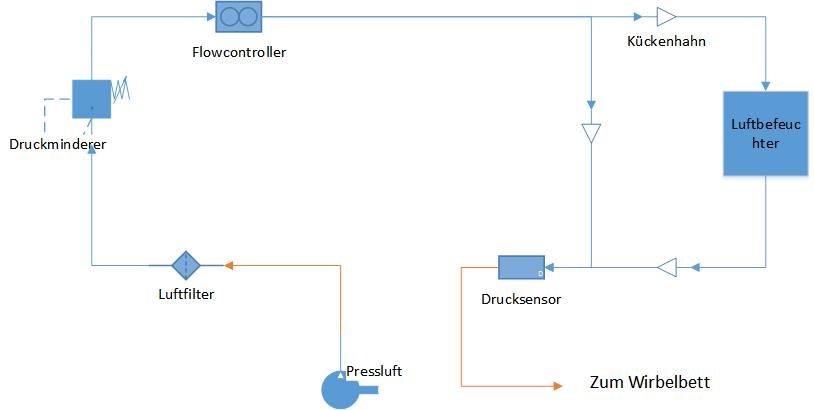
\includegraphics[scale=0.6]{Aufbau_Gassystem.jpg}
		\caption{Schema Gassystem}
	\end{center}
\end{figure}


Um dem Aufbau die nötige Flexibilität zu geben, die beim Umbau zwischen den beiden Versuchsständen nötig ist, wurde das Wirbelbett mit einem Bunaschlauch (\textcolor{orange}{orange}) an das Gassystem angeschlossen. Zudem ist der Anschluss des Gassystems an die Durckluftversorgung mit einem Bunaschlauch gelöst. Sämtliche Rohrleitungen ab dem Luftfilter bis zum Übergang zum Wirbelbett sind aus Edelstahl. \\
Die Ventile, T-Stücke und Verbindungsstücke sind auch aus Edelstahl, da Messing zwar billiger wäre, allerdings auch weicher, was zu Verformungen und höherem Verschleiß führen kann. \\
Abschließend kann gesagt werden, das durch die Wahl der Verrohrung ei luftdichtes Gassystem erreicht wurde. Außerdem ist der Aufbau mit $\SI{000}{m} \cdot \SI{000}{m}$ passend für den Lichtstreuaufbau.


\subsubsection{Luftbefeuchter}

Um die Anforderungen für den Luftbefeuchter zu erfüllen, wurden drei mögliche Lösungen geprüft, dabei war die Größe der Lösung das Hauptaugenmerk.

\paragraph{Swagelok} 

\hfill \\

Von Swagelok gibt es eine Lösung ähnlich dem jetzigen Drucksensor. Über ein spezielles Rohrverbindungsstück kann ein Metallzylinder angeschlossen werden, der senkrecht auf dem Rohr nach oben steht. Dieser wird mit Wasser gefüllt, das von unten mit Luft durchströmt wird und die anschließend oben abgenommen und Richtung Wirbelbett fließt.

\paragraph{Befeuchtung durch Vorbeiströmen}

\hfill \\

In einer anderen Arbeit \cite{Fallturmexperiment} wurde die Luftbefeuchtung realisiert, indem man Luft direkt an einer  Wasseroberfläche vorbeiströmen ließ und die Luft durch Diffusion Wasser aufnahm. 

\paragraph{Eigenbau}
\hfill \\

Eine alternative Methode ist mit gleicher Funktion wie die Lösung von Swagelok, besteht darin einen eigenen Luftbefeuchter zu bauen. 


\paragraph{Auswahl}

\hfill \\

Es wurde sich für die Lösung \glqq Eigenbau\grqq \ entschieden, da die anderen Methoden Mängel aufweisen. Die Lösung von Swagelok ist zum einen sehr teuer, zudem würde bei angeschaltetem Gasfluss Wasser in das System fließen. \\
Die Methode des Vorbeiströmens fiel raus, weil eine zu große Strömfläche gebraucht wurde. Anhand der Formeln aus der Arbeit von Herrn Schmitz, erhielt man eine Fläche von $\SI{50}{cm} \cdot \SI{50}{cm}$. Ein Aufbau dieser Größe ist unmöglich im Lichtstreuaufbau unterzubringen.

\paragraph{Umsetzung}

\hfill \\

Damit der Befeuchter in den Lichtstreuaufbau passt, wurde zu Anfang ein Behältnis ausgewählt, das in den Aufbau passt und dann wurden die für den Befeuchter nötigen Änderungen vorgenommen. Dazu wurde der Kanister mit einem Durchmesser von \SI{22}{cm} und einer Höhe von \SI{50}{cm} (???) auf einer Höhe von \SI{00}{cm} (???) horizontal aufgeschnitten. Nun war es möglich die benötigten Komponenten in dem Behälter unterzubringen. Der schematische Aufbau ist in der unten stehenden Skizze zu sehen: \\

\begin{figure}[h]
	\begin{center}
		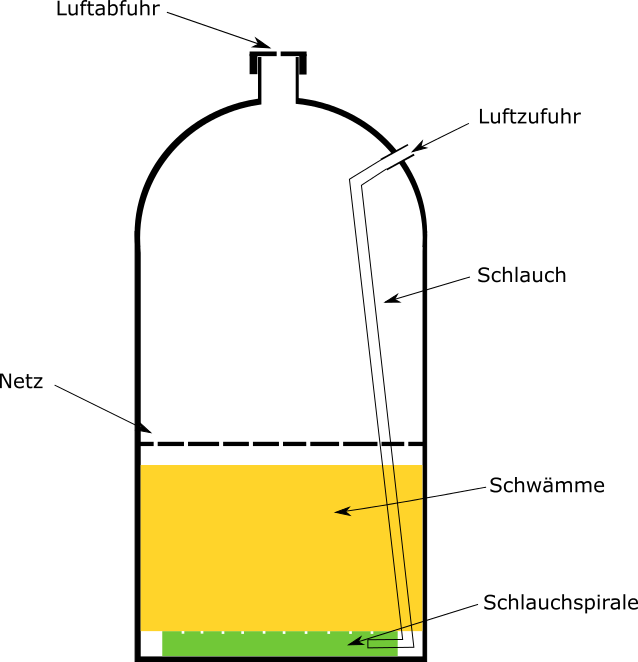
\includegraphics[scale=0.6]{Luftbefeuchter.png}
		\caption{Skizze Luftbefeuchter}
	\end{center}
\end{figure}

Eine weitere Herausforderung war die Luft mit dem geforderten Feuchtigkeitsgrad von $\SI{75}{\%}$ anzureichern. Ein erprobtes Verfahren ist, die Luft durch eine gesättigte Kochsalzlösung zu leiten. Dadurch wird automatisch eine Luftfeuchtigkeit von $\SI{75}{\%}$ erreicht. Die Luft muss allerdings als sehr feine Blasen durch die Kochsalzlösung wandern, da die Steigzeit sonst nicht ausreicht die Luft anzureichern. \\
Dies wurde erreicht, indem die Luft aus einer Schlauchspirale mit feinen Löchern durch eine zweilagige Schicht aus handelsüblichen Küchenschwämmen geleitet wurde. \\
Damit die Schwämme nicht durch den Luftstrom von ihrem Platz weggedrückt werden, wurde $\SI{2}{cm}$ darüber ein Netz gespannt.

\begin{figure}[h]
	\begin{minipage}[hbt]{7cm}
		\centering
		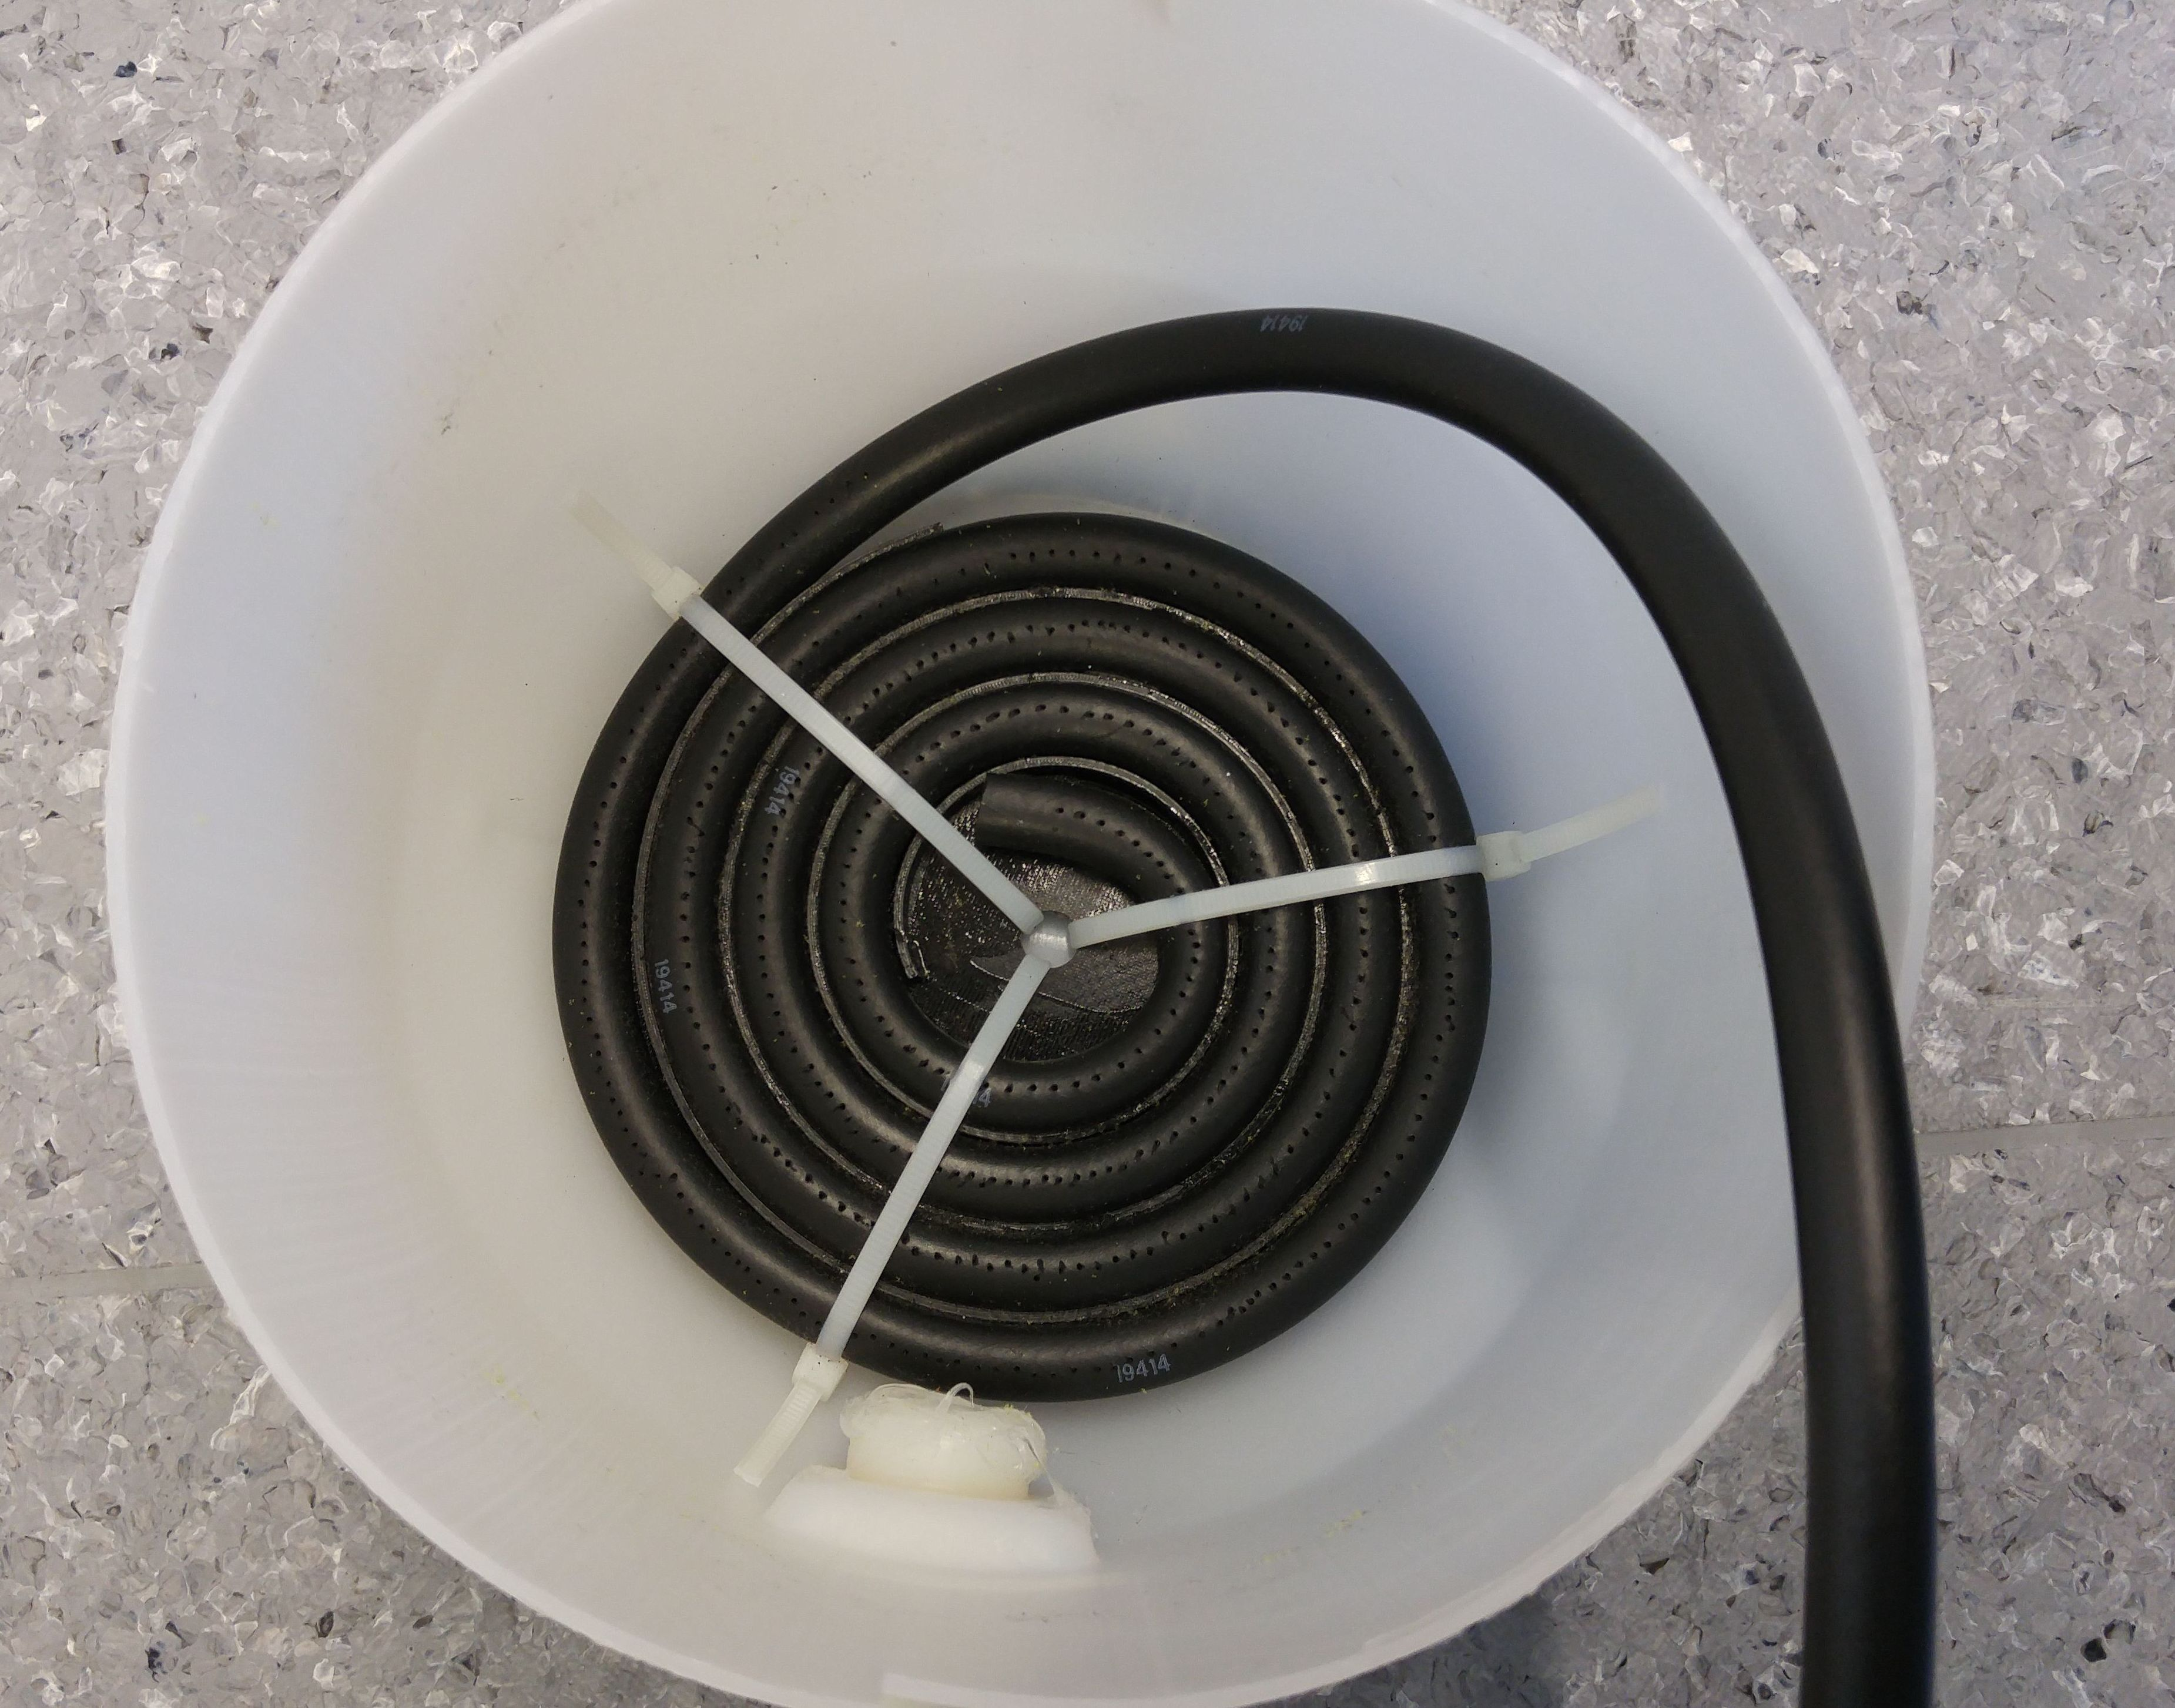
\includegraphics[width=7cm]{Luftbefeuchter_Spirale.jpg}
		\caption{Spirale}
	\end{minipage}
	\hfill
	\begin{minipage}[hbt]{7cm}
		\centering
		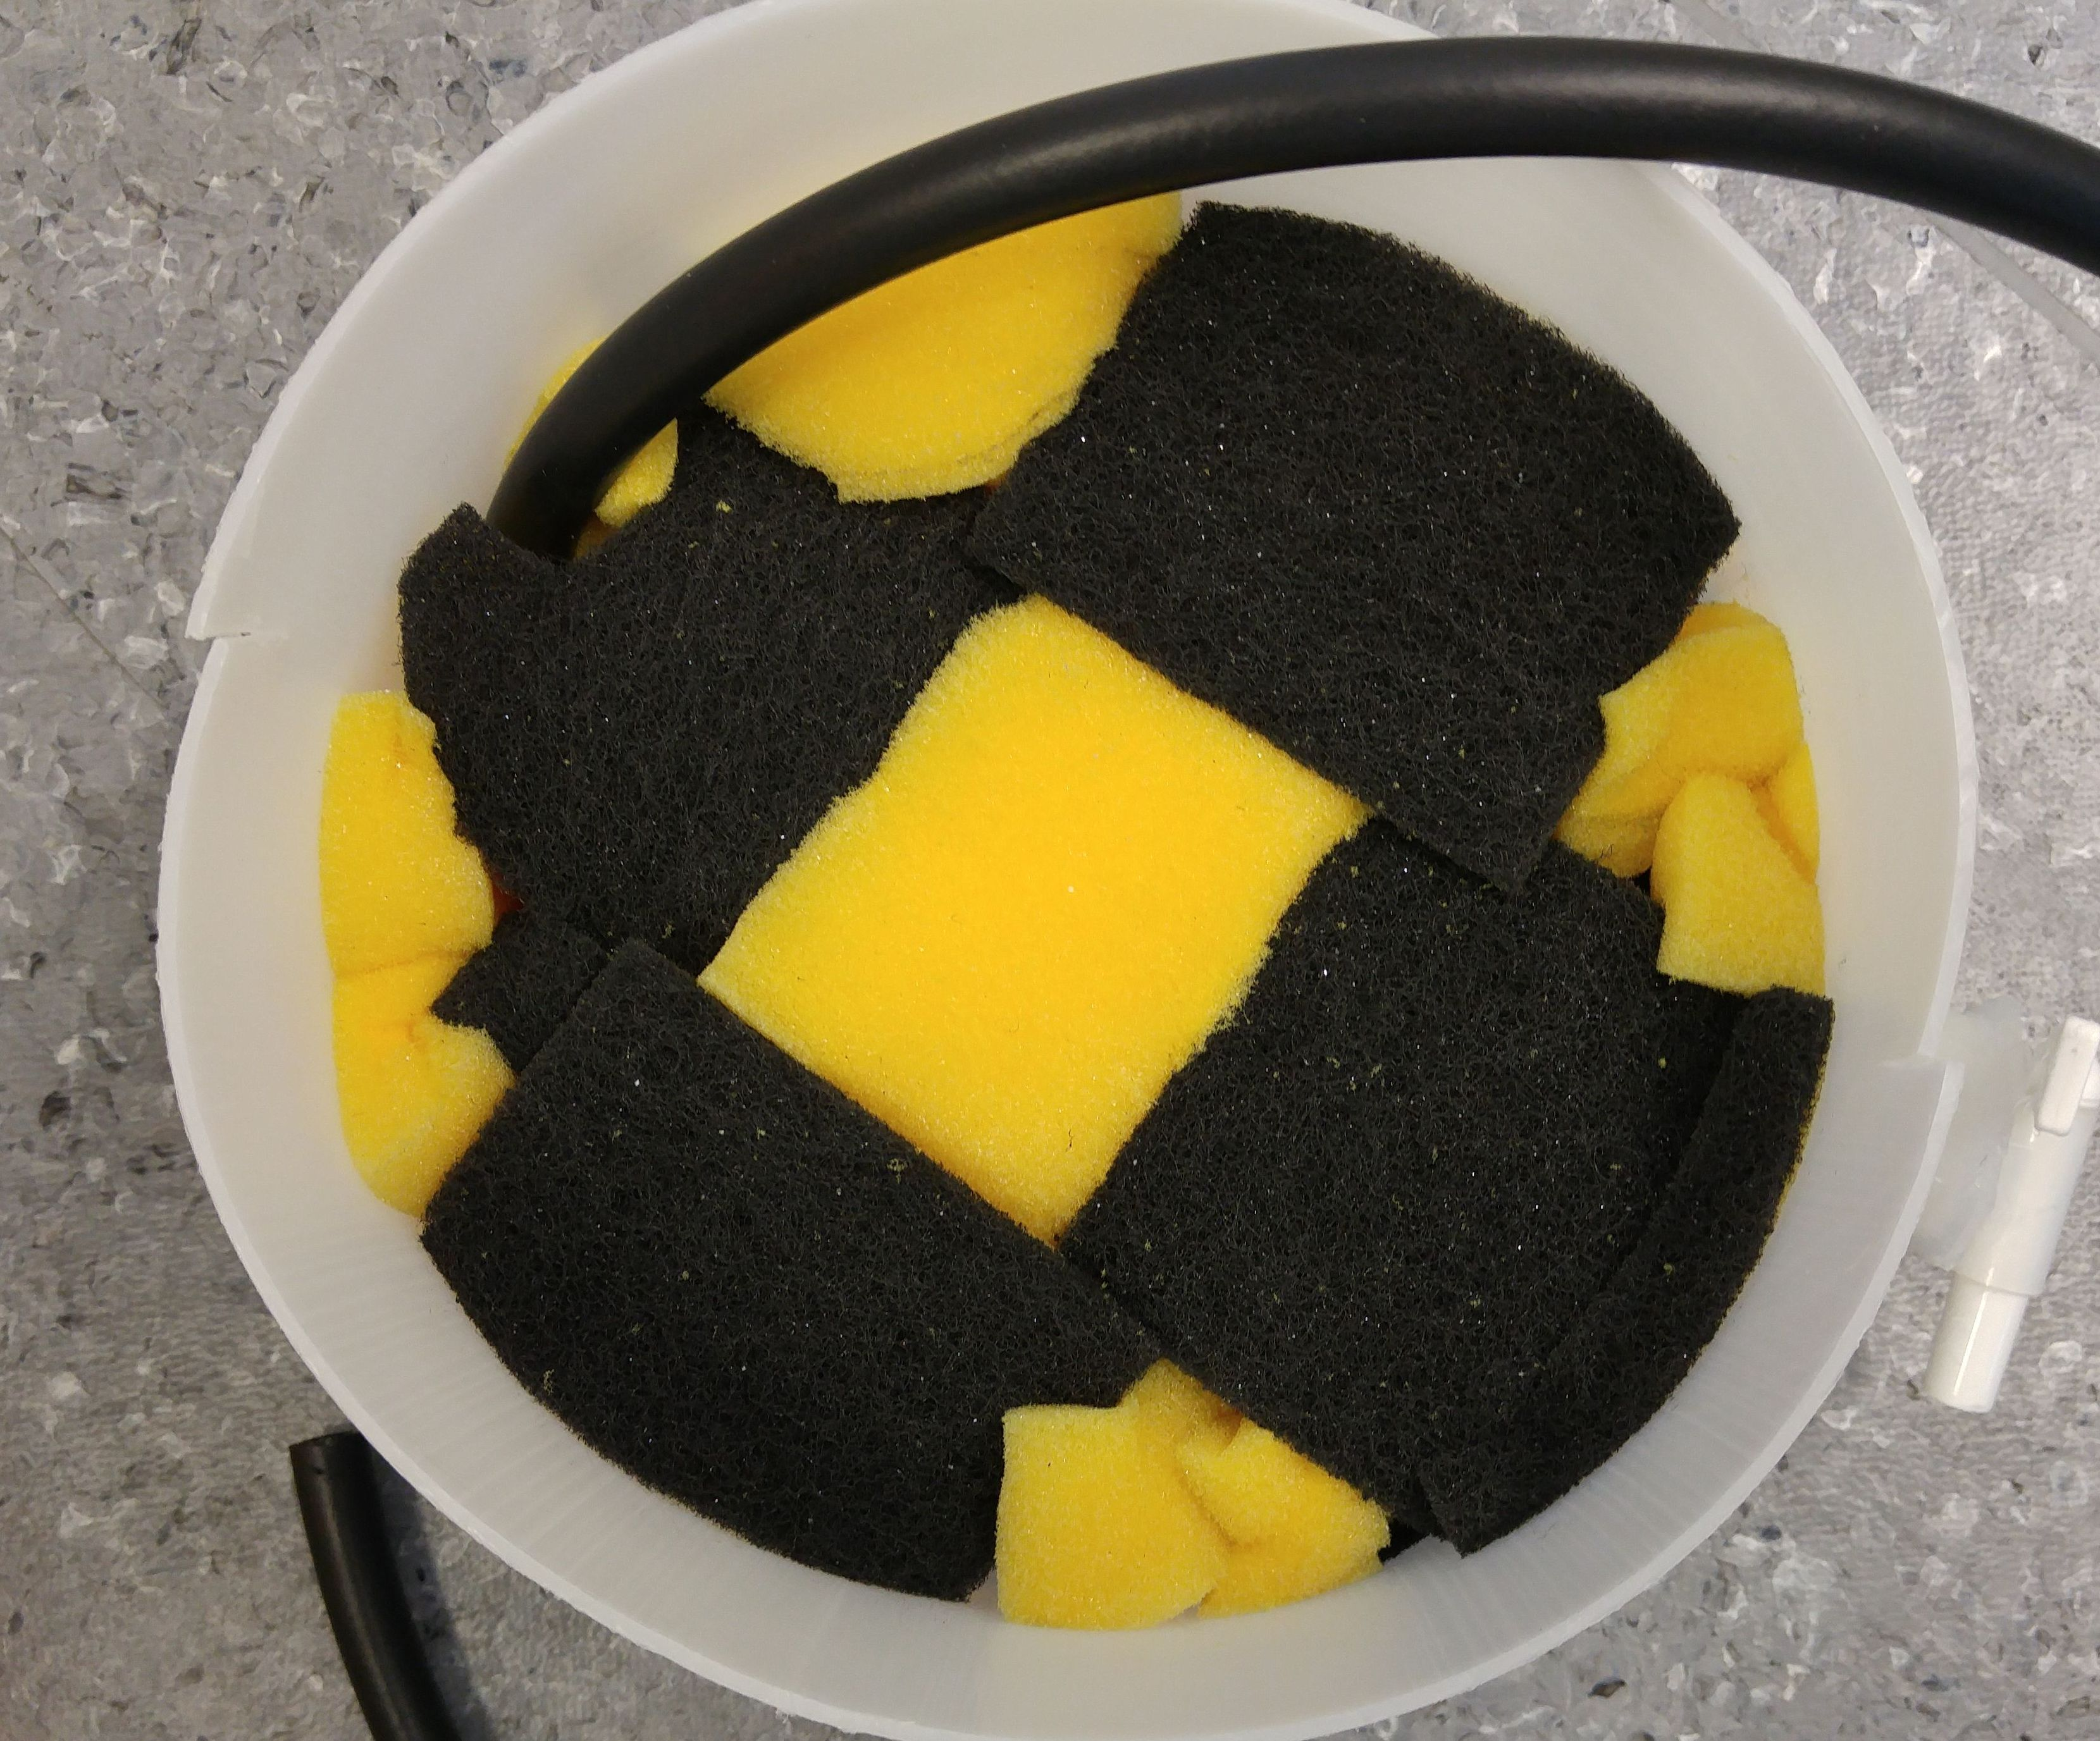
\includegraphics[width=7cm]{Luftbefeuchter_Schwaemme.jpg}
		\caption{Schwämme}
	\end{minipage}
\end{figure}

Anschließend wurde in die obere Hälfte des Behälters eine Kombination aus einem Swagelok \SI{6}{mm} Rohrverbinder und einem Schlauchanschluss eingefügt. So kann man von außen ein Standard \SI{6}{mm} Stahlrohr anschließen und innen den Bunaschlauch für die Spirale. Die Lösung für die Luftabfuhr wurde ähnlich realisiert. Dazu wurde in den Verschluss wiederum ein \SI{6}{mm} Rohrverbinder eingefügt und der Verschluss auf der Innenseite mit einer Schicht Silikon ausgekleidet, sodass man ihn noch auf- und abdrehen kann um Wasser nachzufüllen, gleichzeitig aber die Luftdichtheit gewährleistet ist.


\begin{figure}[h]
	\begin{minipage}[hbt]{7cm}
		\centering
		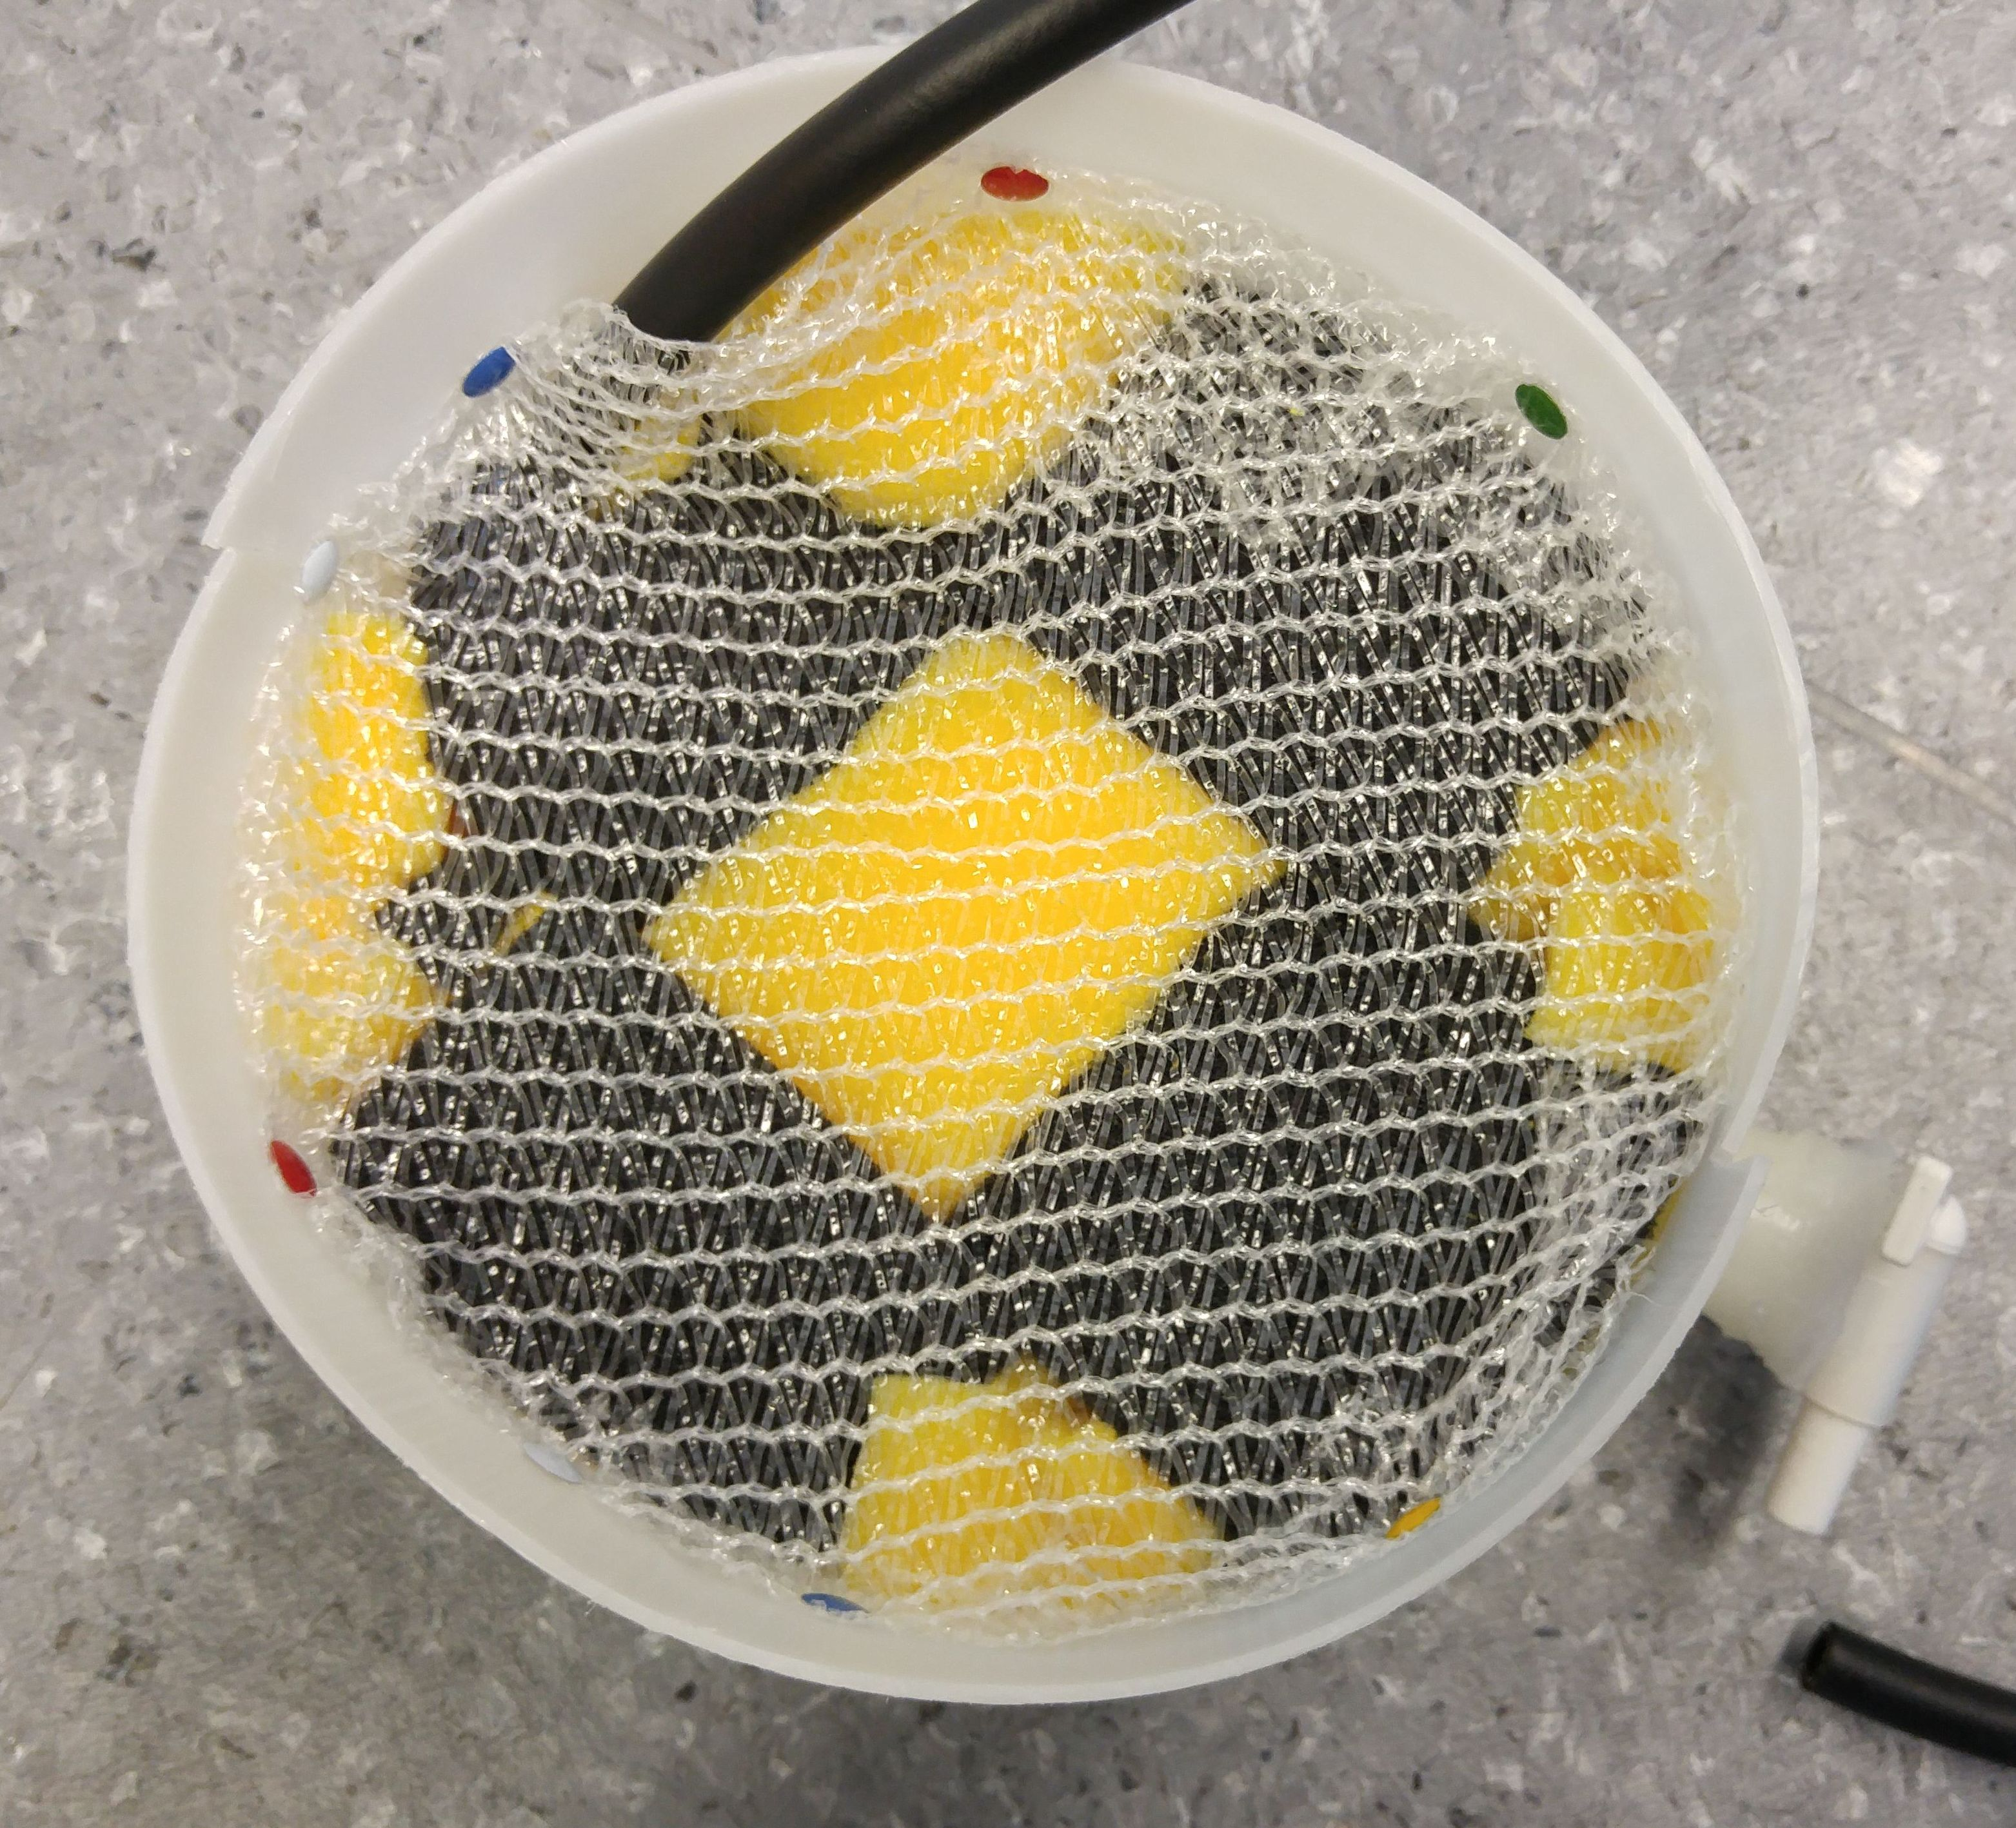
\includegraphics[width=7cm]{Luftbefeuchter_Netz.jpg}
		\caption{Netz}
	\end{minipage}
	\hfill
	\begin{minipage}[hbt]{7cm}
		\centering
		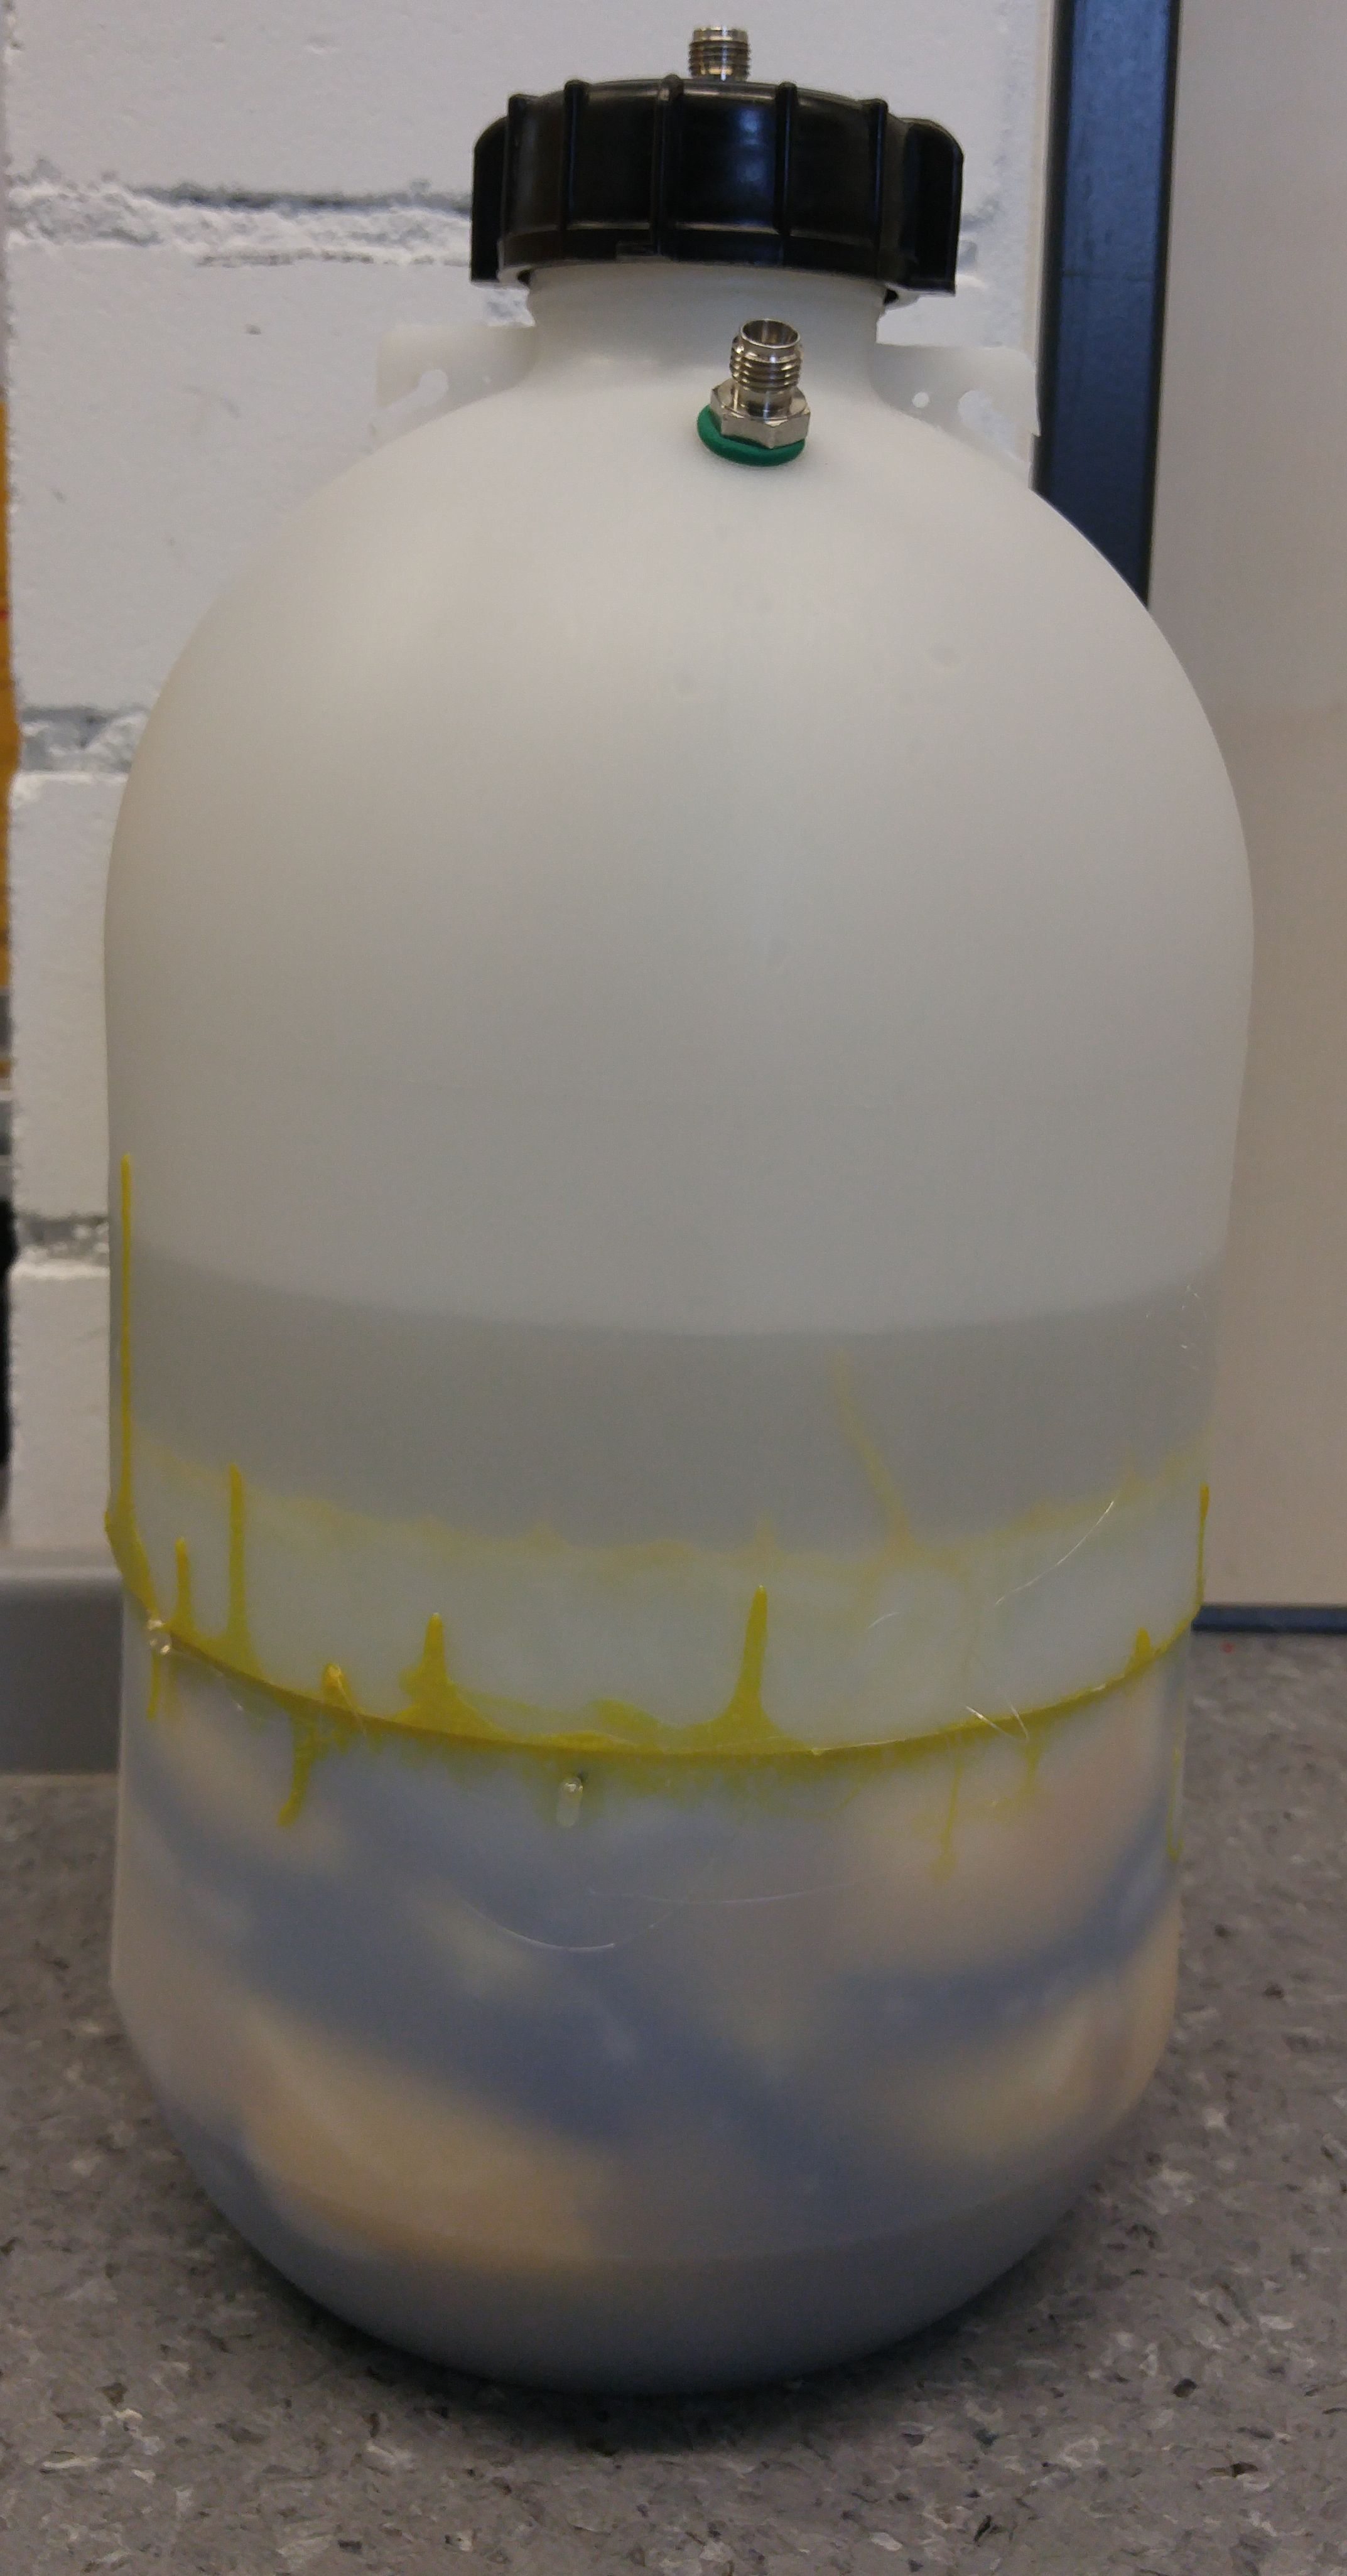
\includegraphics[width=7cm]{Luftbefeuchter_gesamt.jpg}
		\caption{Außenansicht mit eingefülltem Wasser}
	\end{minipage}
\end{figure}

\newpage

\section{AP4 - Wirbelbett}


\subsection{Allgemeine Anforderungen}

Da das bisherige Wirbelbett nicht flexibel genug konfigurierbar war, musste es neu konstruiert werden und dabei möglichst modular werden. Zum einen soll es möglich sein Probenröhrchen von \SI{5}{mm}, \SI{20}{mm}, \SI{30}{mm} und \SI{40}{mm} nutzen zu können. Weiterhin ist es erforderlich sowohl die Probenröhrchen als auch das Probenmaterial einfach und schnell wechseln zu können. Außerdem wurde gefordert, das aus dem Probenröhrchen austretende Partikel aufgefangen werden können. Des weiteren musste ein neuer Filter für den Übergang vom Anschlusszylinder zum Probenröhrchen gefunden werden. 
Eine weitere Anforderung bestand in der Integration eine Ionisators, sodass die durch das Probenröhrchen strömende Luft ionisiert werden kann. Die gesamte Konstruktion muss zudem in den Lichtstreuaufbau passen. \\




\begin{figure}[h]
	\begin{center}
		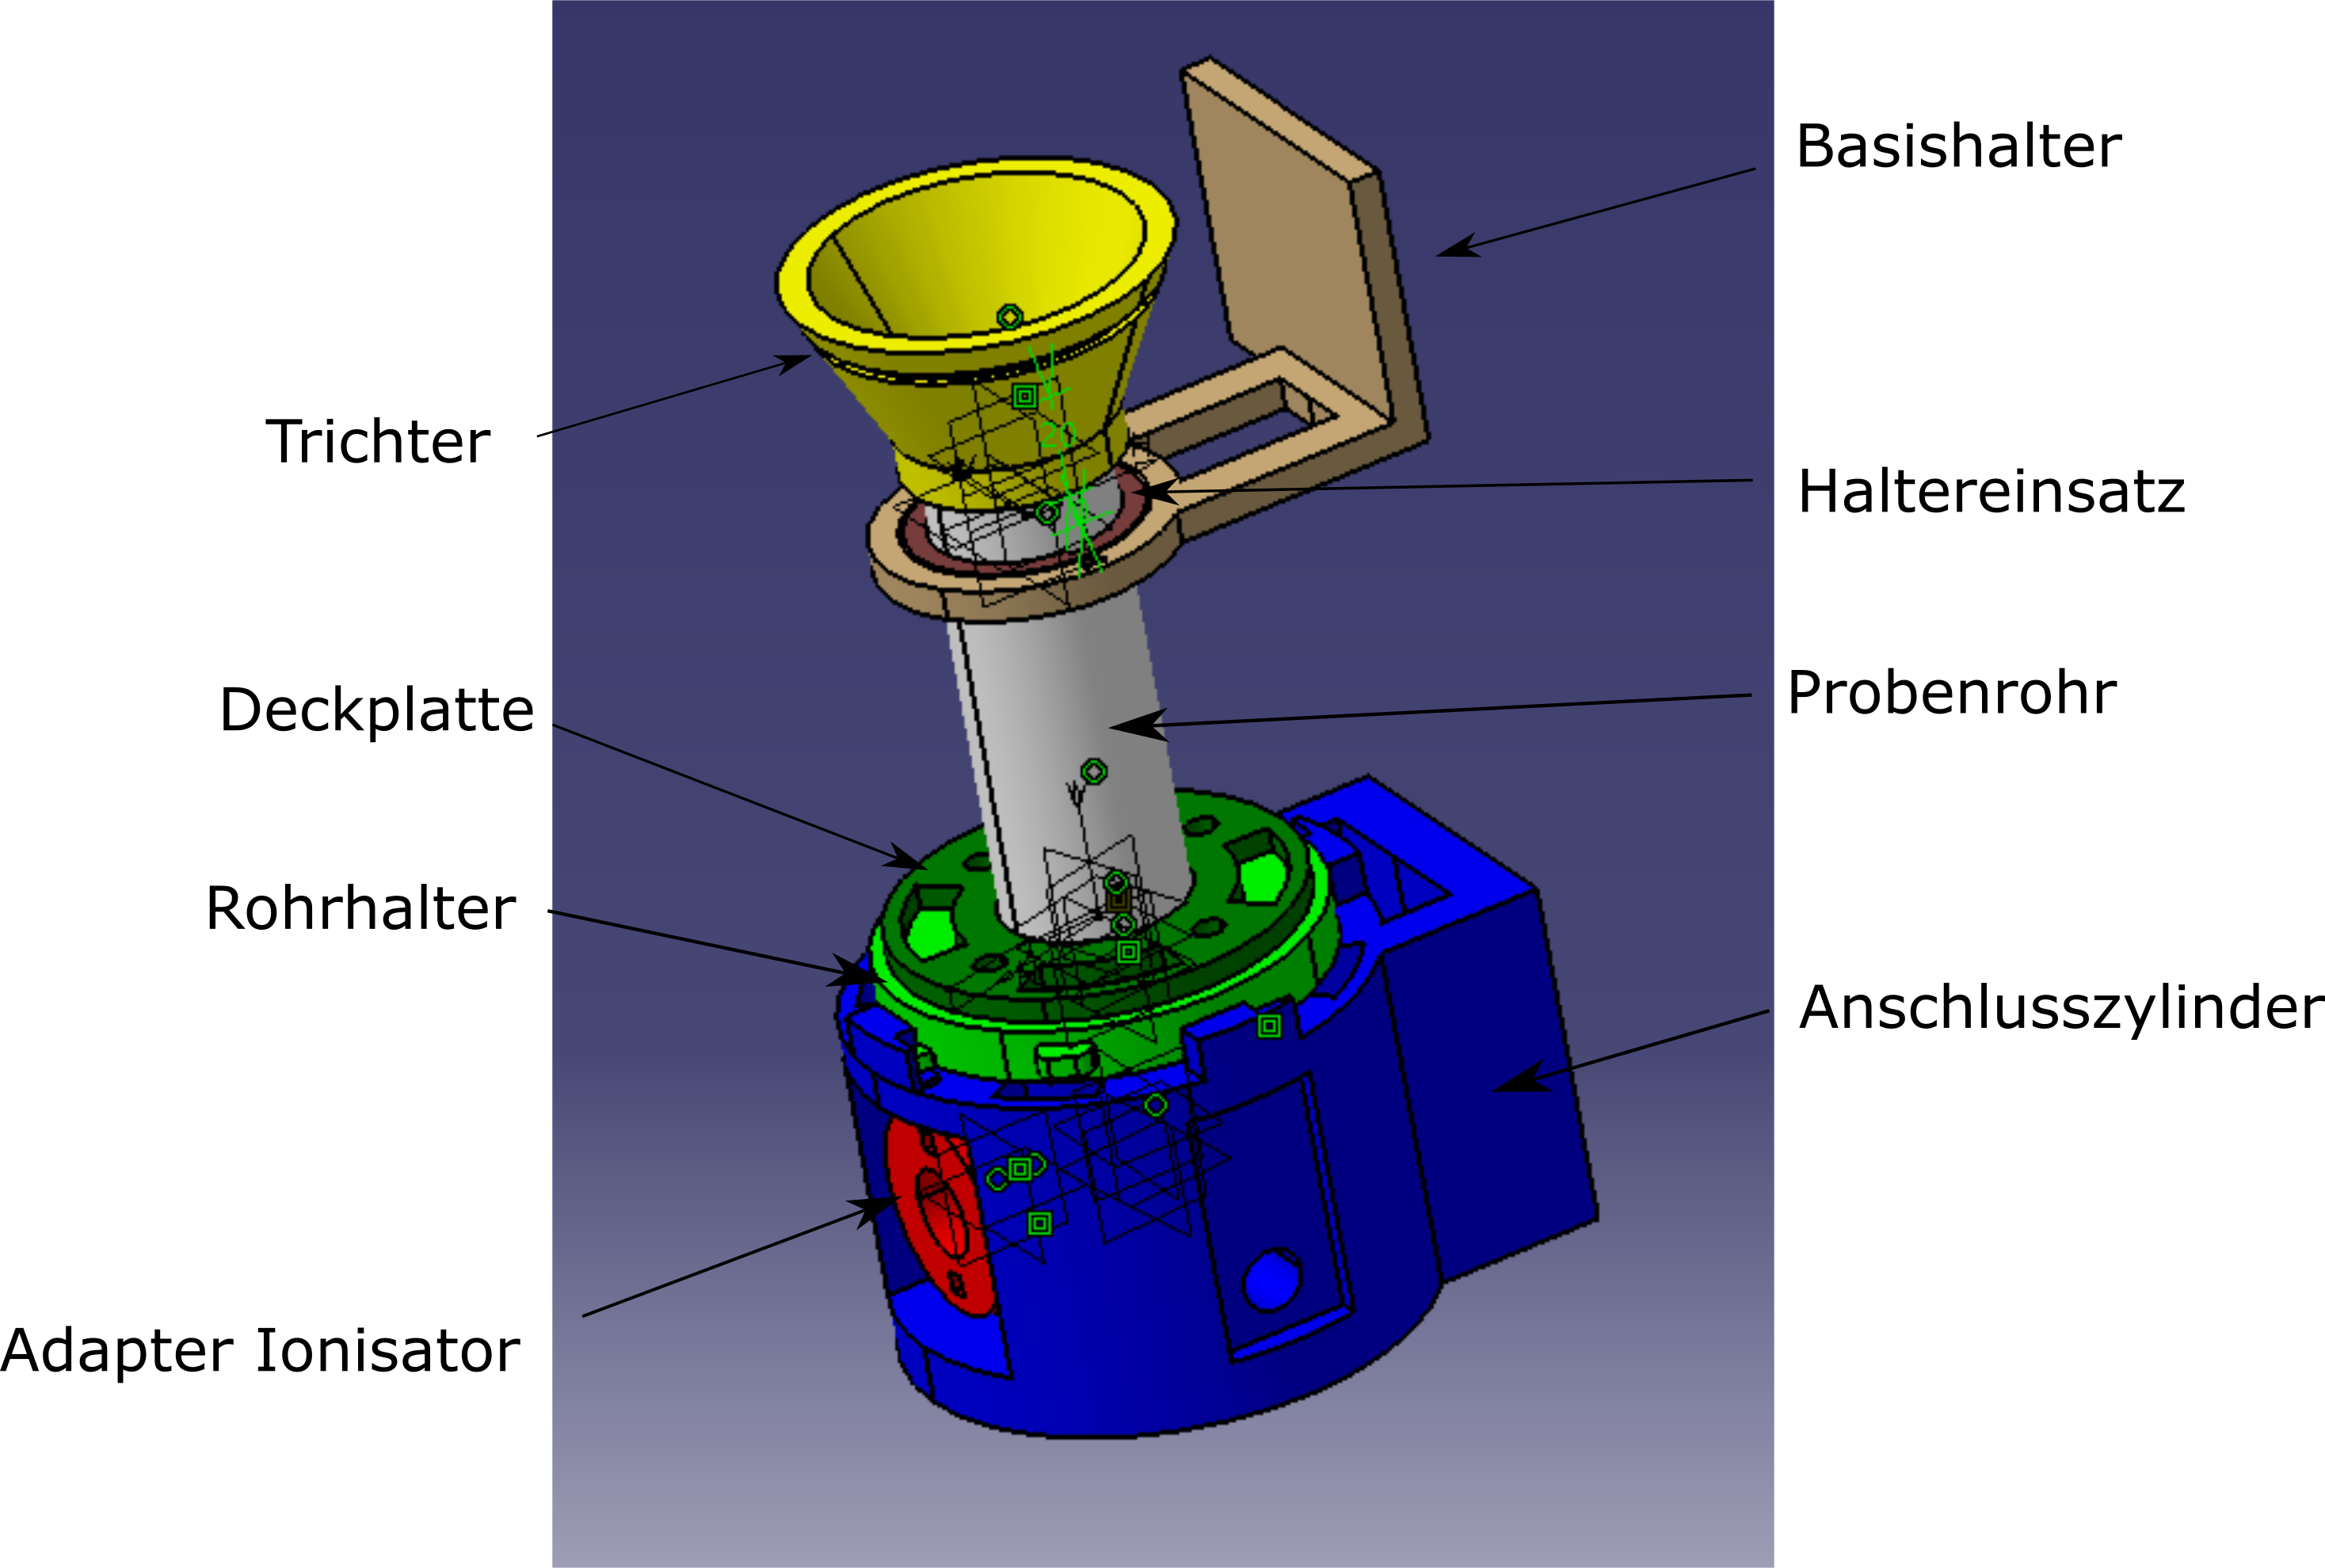
\includegraphics[scale=0.6]{Zusammenbau_fluides_Bett.png}
		\caption{Digitalmodell Wirbelbett}
	\end{center}
\end{figure}


Im folgenden werden die im Bild zu sehenden Bauteile in Abschnitten diskutiert, die sich mit der Methode zum auffangen des Granulats, dem Anschlusszylinder, dem Röhrchenhalter, der Halterung des Wirbelbetts und dem Filter beschäftigen.


\subsection{Methode zum Granulat auffangen}

\subsubsection{Anforderung}

Wie schon in der Einleitung beschrieben, hat ein granulares Medium mehrere Phasen gleichzeitig, von denen die oberste die Gasphase ist. Je nach Füllstand und Gasfluss des Messröhrchens kann es nun passieren, das einzelne Partikel oben aus dem Röhrchen hinausfliegen. Außerdem braucht es eine Absicherung gegen Fehlbedienung, sodass bei zu hohem Gasstrom kein Granulat aus dem Probenröchrchen austritt.

\subsubsection{Auswahl}

\paragraph{Fliehkraftabscheider} 

\hfill \\

Ein sehr beliebtes Produkt, um Luft von Partikeln zu säubern, ist der Fliehkraftabscheider oder Zyklon. Dieser basiert auf dem Prinzip, das die Luft immer weiter beschleunigt wird und die darin enthaltenen Partikel an die Wand gedrückt werden und schließlich nach unten raus fallen. \\


\begin{figure}[h]
	\begin{center}
		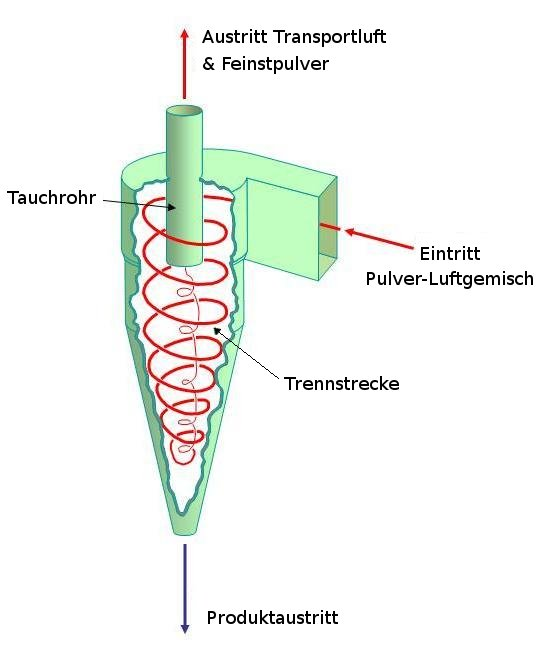
\includegraphics[scale=0.5]{Umsetzung_Fliehkraftabscheider.jpg}
		\caption{Fliehkraftabscheider: Quelle Wikipedia}
	\end{center}
\end{figure}



Das Problem bei diesem Bauteil besteht darin, das die kommerziell erhältlichen Versionen sehr teuer sind und zudem zu groß für unserem Aufbau passen. \\
Weiterhin wäre ein erheblicher Konstruktionsaufwand nötig, um einen eigenen Zyklon zu bauen, da die Luft in unserem Versuch von unten kommt, der Zyklon sie aber von der Seite braucht. \\

\paragraph{Trichter}

\hfill \\

Eine Alternative dazu ist ein Trichter, der den Querschnitt aufweitet und so den Gasstrom verlangsamt. Aus Kosten und den oben beschriebenen Konstruktionsproblemen wurde entschieden einen Trichter zu entwerfen.



\subsubsection{Umsetzung}

Um den Gasstrom zu verlangsamen und gleichzeitig das Einfüllen des Granulats zu erleichtern, wurde jeweils ein Trichter konstruiert, der passgenau mit dem Innendurchmesser jedes Probenröhrchens abschließt und zudem den Querschnitt verdoppelt. \\
Wie man anhand der Formel $v_a = \frac{Q}{A}$ \cite{Grollius2012} sehen kann, ist die Geschwindigkeit des Gasstrom direkt proportional zum Querschnitt des Rohrs. Wenn man also den Querschnitt verdoppelt, dann viertelt man die Geschwindigkeit des Gasstroms. Dies wurde für jeden Durchmesser gemacht. Man könnte zwar bei gleicher Höhe auch die Querschnitte unter \SI{40}{mm} auf \SI{80}{mm} aufweiten, allerdings bringt das stömungstechnisch nicht viel, da sich der Luftstrom nicht so schnell so stark aufweiten kann. \\
Zudem wurde ein abnehmbarer Filter oben auf den Trichter gespannt, um einen rudimentären Schutz gegen austretende Partikel bei Fehlbedienung zu gewährleisten.

Hier Konstruktionsskizze einfügen


\subsection{Anschlusszylinder}

\subsubsection{Anforderungen}

Im Prinzip gab es im vorigen Aufbau auch schon einen Anschlusszylinder, allerdings brauchte man mehr Features und mehr Flexibilität. Das Ziel bei diesem Zylinder war den Anschluss an das Gassystem zu haben und eine Halterung für die verschieden großen Röhrchen zu haben. Zudem sollte gewährleistet werden, das ein Ionisator ein den Luftstrom eingebracht werden kann.


\subsubsection{Umsetzung}

Der Kern des Anschlusszylinders ist die $\SI{40}{mm}$ breite Röhre, damit Röhrchendurchmesser bis $\SI{40}{mm}$ mit einem laminaren Gasstrom versorgt werden können. \\
Auf der Oberseite befindet sich eine Nut in die der O-Ring zum Abdichten der Verbindung Anschlusszylinder-Röhrchenhalter. Damit diese Verbindung dicht ist, befindet sich auf der Oberseite zudem ein Arretierungsmechanismus in den der Röhrchenhalter eingedreht wird. Zudem garantiert dieser Mechanismus ein einfaches und schnelles lösen der Komponenten.


Hier Doppelbild einfügen


In der Frontansicht sieht man den Einlass mit Arretierung für den Ionisator. Zur Montage wird die Spitze des Ionisator in einen Adapter gesteckt und dieser Adapter mittels drehen arretiert. Die Luftdichtheit wird durch einen O-Ring aus Gummi (Shore Härte 50) erreicht. \\
In der Seitenansicht wird der Anschluss für das Gassystem sichtbar. Hier wurde ein Swagelockverbinder mit Gummi O-Ring in das Plastik geschraubt und der Adapter für den Bunaschlauch daran angeschlossen.


\subsection{Röhrchenhalter}

\paragraph{Umsetzung}

\hfill \\

Der Röhrchenhalter besteht aus drei Teilen, eins dient zur Verbinung mit dem Anschlusszylinder und das andere sorgt dafür, dass die Dichtung an Ort und Stelle gehalten wird. \\
Die beiden Teile werden durch vier M6 Schrauben verbunden, damit der Druck auf den dichtenden O-Ring möglichst gleichmäßig verteilt ist. \\
Im oberen Teil sind zudem vier Aussparungen, die die Stabilität nicht beeinträchtigen aber Material sparen. 

Hier Doppelbild einfügen


Der dritte Teil des Halters sorgt dafür, dass das Röhrchen nicht seitlich verkippt werden kann und es dadurch zu Undichtigkeiten kommt. Damit diese Halterung nicht für jedes Röhrchen seperat montiert werden muss, wurde ein universelles Ringsystem entworfen. Das Basisteil wird am Schanier festgeschraubt und hat $\SI{40}{mm}$ Durchmesser. In das Basisteil können nur weitere Ringe eingesetzt werden, damit auch die Durchmesser $30,20,5\SI{}{\ mm}$ einen guten Halt haben.


\subsection{Halterung Wirbelbett}

\subsubsection{Lichtstreuaufbau}


\paragraph{Anforderungen}

\hfill \\
Die Aufgabe bestand darin, das Wirbelbett so in den Aufbau zu integrieren, sodass weder die Rotationsfähigkeit vermindert, noch der Aufbau verändert wird. Zudem sollte die Höhe des Wirbelbetts rudimentär geändert werden und die Position in der Horizontalen im Submilimeterbereich eingestellt werden können. 


\paragraph{Umsetzung}
\hfill \\
Um den Anforderungen gerecht zu werden, wurde eine Konstruktion aus zwei L-förmigen Teilen gewählt. 

\begin{figure}[h]
	\begin{minipage}[hbt]{7cm}
		\centering
		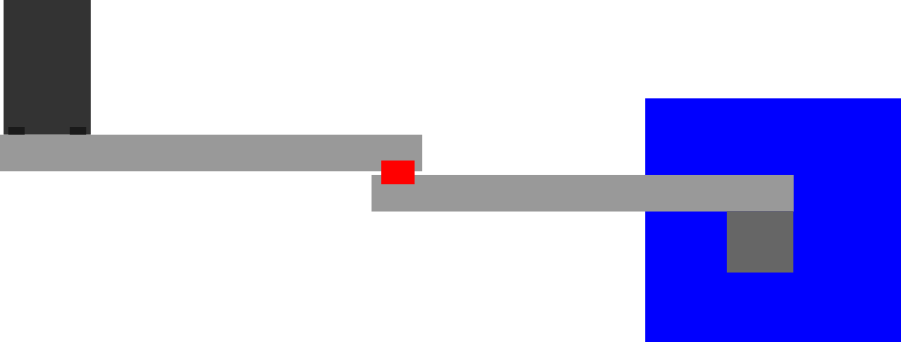
\includegraphics[width=7cm]{Halterung_Lichtstreu_Vogel.png}
		\caption{Draufsicht}
	\end{minipage}
	\hfill
	\begin{minipage}[hbt]{7cm}
		\centering
		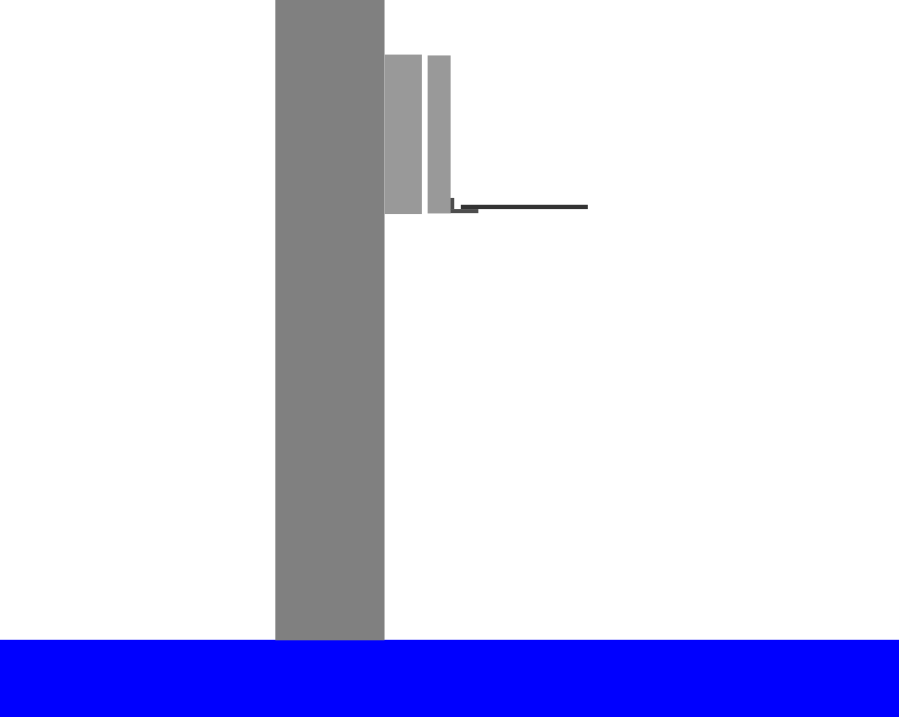
\includegraphics[width=7cm]{Halterung_Lichtstreu_Seite.png}
		\caption{Seitenansicht}
	\end{minipage}
\end{figure}


In der Draufsicht sieht man, das zum Verschieben nach links und rechts zwei durch eine Laborklemme (rot) gegeneinander verschiebbare Träger genutzt wurden. Ans Ende es linken Trägers wurde mittels zwei Winkeln die Halteplatte für das Wirbelbett montiert. Auf der Halteplatte kann das Wirbelbett mit der Mikrometerschraube exakt in den Laserstrahl gefahren werden.





\subsection{Filter}

\paragraph{Anforderungen}
\hfill \\
Das Ziel bestand darin einen Filter zu finden, der, im Gegensatz zu dem vorher verwendeten Schwamm, immer die gleichen Eigenschaften aufweist, auch wenn man ihn austauscht. Zudem muss der Filter durchlässig genug sein um bis zu $\SI{3000}{l/h}$ Luft durchzulassen, ohne zu reißen. Zugleich müssen die Poren fein genug sein, damit die Partikel des kleinsten Granulats nicht hindurch fallen. Außerdem muss der Filter dünn genug sein, damit der die Höhe der Konstruktion nicht negativ beeinflusst, da es beim Lichtstreuaufbeu eine Höhenbegrenzung gibt. Weiterhin musste der Filter hydrophob und antistatisch sein, sodass er bei Zuschaltung des Luftbefeuchters kein Wasser aufnimmt und dadurch verstopft und sich nicht statisch aufläd.


\paragraph{Auswahl}
\hfill \\
Um einen geeigneten Filter zu finden wurde sich mit den Herstellern Merk Millipore, Sartorius und Nitto in Verbindung gesetzt. Am Schluss hatten wie die Auswahl zwischen folgenden Filtern:


\begin{center}
			\begin{tabular}{l|c|c|c}
				& Sartorius & Merck Millipore & Nitto \\
				\hline
				Porengröße [$\mu$m] & 0,45  & 10    & 24 \\
				Dicke[$\mu$m] & 125 & 130 & 500 \\
				Porösität[$\%$] & 75    & 60    & 38 \\
				Luftdurchlass [$l/min \cdot cm^2$] & 20    & 14    & 0,09 \\
				antistatisch & ja    & ja    & ja \\
				hydrophob & ja    & ja    & ja \\
				Material & PVDF\footnotemark[1]  & PTFE\footnotemark[2]  & PE\footnotemark[3] \\
			\end{tabular}	
\end{center}

\footnotetext[1]{Polyvinylidenfluorid}
\footnotetext[2]{Polytetrafluorethylen}
\footnotetext[3]{Polyethylen}

\vspace{0.5cm}

Es wurde sich für die Membran von Sartorius entschieden, weil sie alle Anforderungen erfüllt und in allen Belangen besser ist als die beiden Alternativen. Damit die Membran nicht verrutscht wurde ein jeweils passendes Stück auf die Probenröhrchen geklebt. So ist auch sicher gestellt, das kein Granulat unabsichtlich in den Anschlusszylinder fällt.



\section{Bewertung}


\section{Ausblick}












